\documentclass[a4paper]{article}
\usepackage{a4wide}
\usepackage[english]{babel}
\usepackage{hyperref}

\usepackage{todonotes}

%Accenten
\usepackage[utf8]{inputenc} 
\usepackage[T1]{fontenc}

% Biblio
\usepackage{csquotes}
\usepackage[backend=biber, bibencoding=utf8]{biblatex}

%Code
\usepackage{listings}
\usepackage{color}

%Math
\usepackage{mathtools}
\usepackage{amsmath}
\usepackage{amsfonts}
\usepackage{amssymb}
\usepackage{siunitx}
\sisetup{output-exponent-marker=e, bracket-negative-numbers, open-bracket={\text{-}}, close-bracket={}, round-mode=figures,round-precision=3, scientific-notation=true}

%Plaatjes
\usepackage{graphicx}
\usepackage[small,bf]{caption}
\usepackage{subcaption}
\usepackage[export]{adjustbox}

% Code lay-out
\definecolor{light-gray}{gray}{0.95}
\usepackage{courier}
\lstset{language=Python, 
	tabsize = 4, 	
	columns=flexible, 
	breaklines = true, 
	backgroundcolor=\color{light-gray},
	keepspaces=true,
	showspaces=false,
	showstringspaces=false,
	basicstyle=\scriptsize\ttfamily
}

\renewcommand{\t}[1]{\lstinline[basicstyle=\normalsize\ttfamily]{#1}}

% General lay-out
\renewcommand{\thesection}{\Alph{section}}
\addto\extrasenglish{%
  \renewcommand{\sectionautorefname}{Assignment}%
}

%Math
\renewcommand{\vec}[1]{\ensuremath{\boldsymbol{#1}}}
\providecommand{\abs}[1]{\lvert#1\rvert}
\providecommand{\norm}[1]{\lVert#1\rVert}

%Short cuts
\newcommand{\p}[1]{\ensuremath{\vec{P_#1}}}
\renewcommand{\vec}[1]{\ensuremath{\mathbf{#1}}}
\renewcommand{\v}[1]{\ensuremath{\vec{v_#1}}}

\title{Geometric Algorithms\\Assignment 4}
\author{Laura Baakman (s1869140)}

\begin{document}

\todo{Code regelnummers checken!}

\maketitle

\section{~}
\label{s:a}
%!TEX root = practicum3.tex
\subsection*{Point in Triangle}

% Theory
We try to determine if the point \vec{Q} lies in the triangle defined by the points $\vec{P_1}$, $\vec{P_2}$ and $\vec{P_3}$. To this end we define the vectors $\vec{v}_1 = \vec{P_2} - \vec{P_1}$ and $\vec{v_2} = \vec{P_3} - \vec{P_1}$, see \autoref{fig:a:triangle_point}. Each point $\vec{P}$ inside the grey area in this figure can be described as:
\begin{equation} \label{eq:a:trianglePointEquation}
	\vec{P} = \vec{P_1} + a \cdot \vec{v_1} + b \cdot \vec{v_2}.
\end{equation}
For all points to the right of \vec{P_1} $a > 0$ and $b > 0$. The points that define the triangle can all be expressed according to \eqref{eq:a:trianglePointEquation}:
\begin{align}
	\vec{P_1} &= \vec{P_1} + 0 \cdot \vec{v_1} + 0 \cdot \vec{v_2} \label{eq:a:p1}\\ 
	\vec{P_2} &= \vec{P_1} + 1 \cdot \vec{v_1} + 0 \cdot \vec{v_2} \label{eq:a:p2}\\ 
	\vec{P_3} &= \vec{P_1} + 0 \cdot \vec{v_1} + 1 \cdot \vec{v_2} \label{eq:a:p3}.
\end{align}
Based on these \eqref{eq:a:p1} through \eqref{eq:a:p3} we find that a point \vec{Q} lies on the triangle if it can be expressed according to \eqref{eq:a:trianglePointEquation} with $a,b \in (0,1)$ and with $a + b < 1$. 

Solving the resulting equation with Mathematica, see \autoref{lst:a:pointInTriangleMathematica}, gives us expressions for $a$ and $b$, namely:
	\begin{align}
	a &= -\frac{-\vec{P_{1,0}} \vec{P_{3,1}}+\vec{P_{1,0}} \vec{Q1}+\vec{P_{1,1}} \vec{P_{3,0}}-\vec{P_{1,1}}
   \vec{Q_0} - \vec{P_{3,0}} \cdot \vec{Q_1}+\vec{P_{3,1}} \cdot \vec{Q_0}}{ - \vec{P_{1,0}}
   \vec{P_{2,1}}+\vec{P_{1,0}} \cdot \vec{P_{3,1}}+\vec{P_{1,1}} \cdot \vec{P_{20}} - \vec{P_{1,1}}
   \vec{P_{3,0}} - \vec{P_{2,0}} \cdot \vec{P_{3,1}}+\vec{P_{2,1}} \cdot \vec{P_{3,0}}}\label{eq:a:a}\\
	b &=  - \frac{ - \vec{P_{1,0}} \cdot \vec{P_{2,1}}+\vec{P_{1,0}} \cdot \vec{Q_1}+\vec{P_{1,1}} \cdot \vec{P_{2,0}} - \vec{P_{1,1}}
   \vec{Q_0} - \vec{P_{2,0}} \cdot \vec{Q_1}+\vec{P_{2,1}} \cdot \vec{Q_0}}{\vec{P_{1,0}}
   \vec{P_{2,1}} - \vec{P_{1,0}} \cdot \vec{P_{3,1}} - \vec{P_{1,1}} \cdot \vec{P_{2,0}}+\vec{P_{1,1}}
   \vec{P_{3,0}}+\vec{P_{2,0}} \cdot \vec{P_{3,1}} - \vec{P_{2,1}} \cdot \vec{P_{3,0}}}\label{eq:a:b}
	\end{align}
where \vec{P_{r,s}} represents the $s$'th element of the point $r$ and \vec{Q_t} repsents the $t$'th element of the point \vec{Q}.

In \eqref{eq:a:a} and \eqref{eq:a:b} are the same, this is the magnitude of the $\vec{v_1} \times \vec{v_2}$ if we represent the vectors as three dimensional by adding a $z$-coordinate of zero. If that cross product is zero $\vec{v_1}$ and $\vec{v_2}$ are parallel and thus the point \vec{Q} cannot be represented according to \eqref{eq:a:trianglePointEquation}.

	\begin{lstlisting}[float, language=Mathematica, label={lst:a:pointInTriangleMathematica}, caption={Mathematica code used to compute the to compute $a$ and $b$.}]
p1 = {p10, p11};
p2 = {p20, p21};
p3 = {p30, p31};
v1 = p2 - p1;
v2 = p3 - p1;

p4 = p1 + a * v1 + b * v2;
p41 = Part[p4, 1] == Q0;
p42 = Part[p4, 2] == pp1;
solution = Solve[{p41, p42}, {a, b}]
	\end{lstlisting}

\begin{figure}
	\centering
	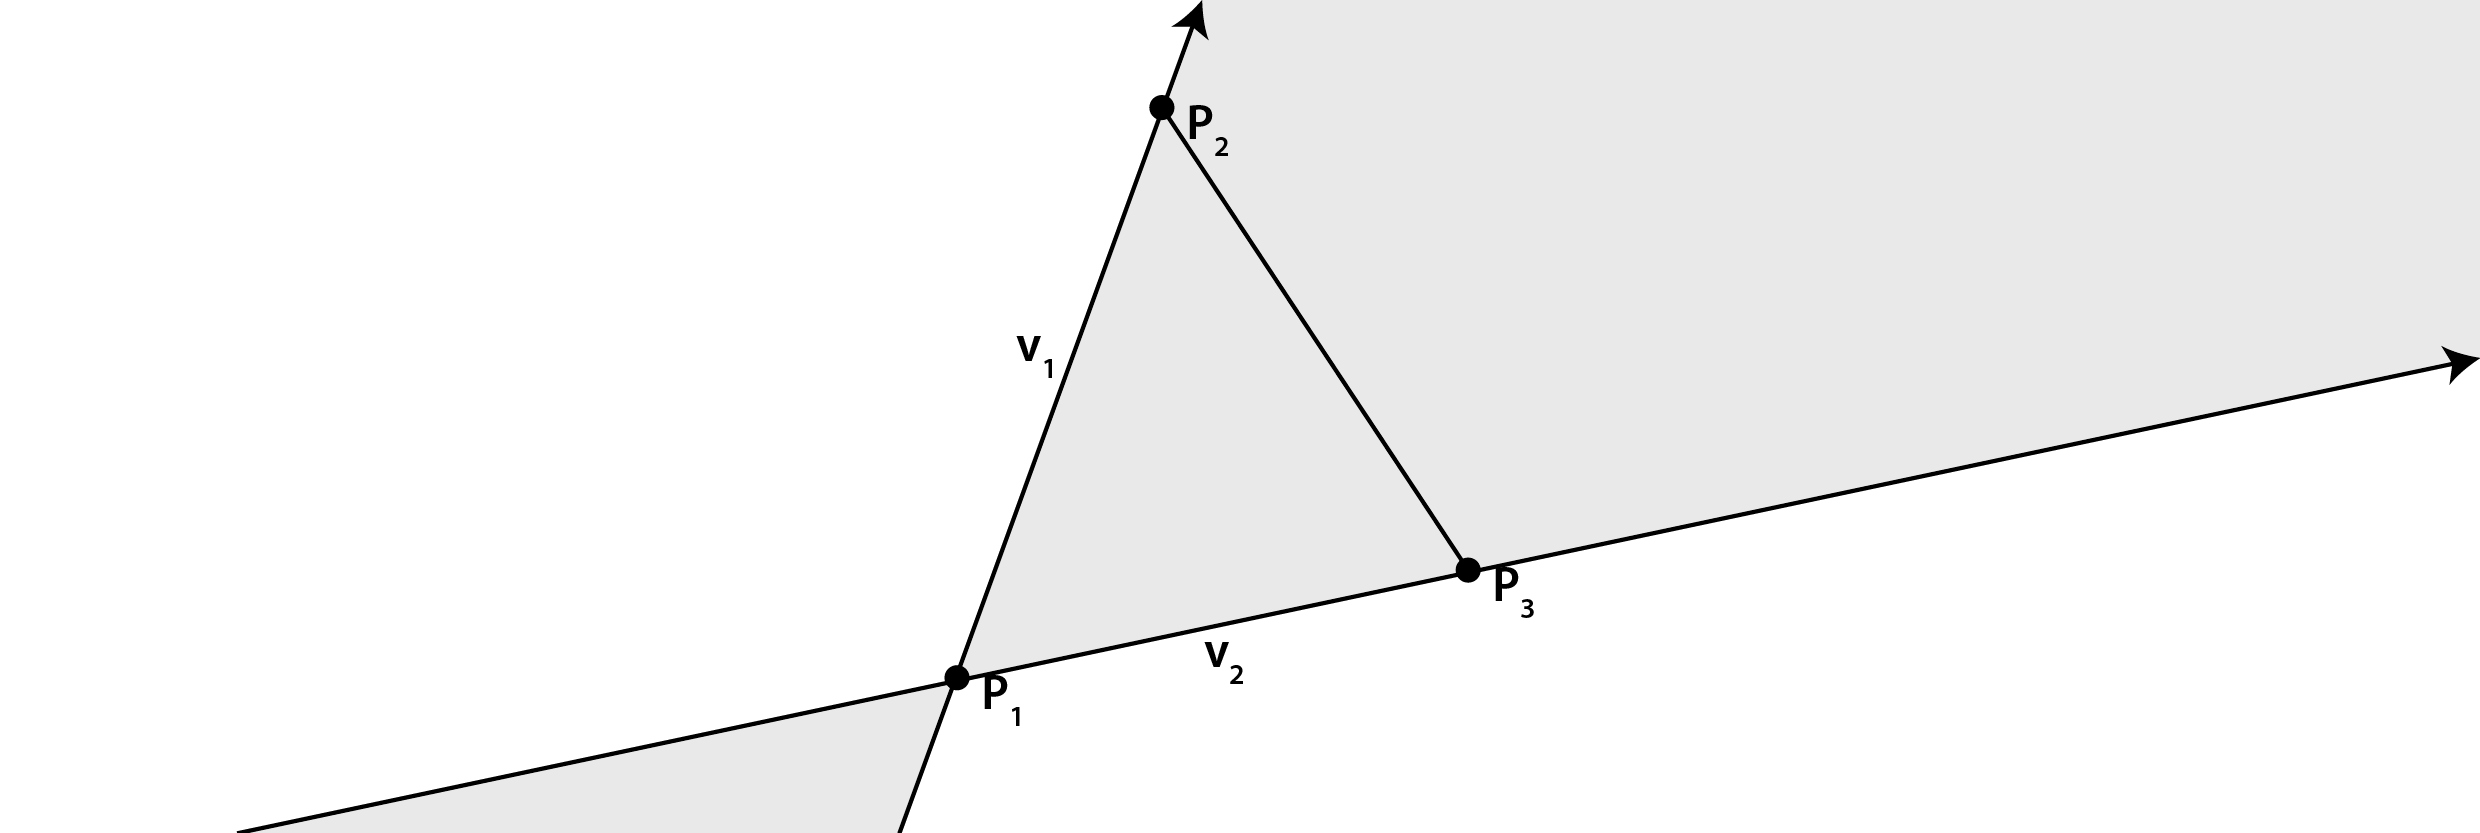
\includegraphics[width=0.9\textwidth, frame]{./img/1_triangle_point-01}
	\caption{A triangle defined by the points $\vec{P_1}$, $\vec{P_2}$ and $\vec{P_3}$, with the vectors $\vec{v_1}$ and $\vec{v_2}$. The grey area covers all points that can be described according to \eqref{eq:a:trianglePointEquation}.}
	\label{fig:a:triangle_point}
\end{figure}




\subsection{Finding the Triangle}


\section{~}
\label{s:b}
%!TEX root = practicum1.tex
\begin{figure}
	\centering
	\begin{subfigure}[b]{0.3\textwidth}
		\centering
		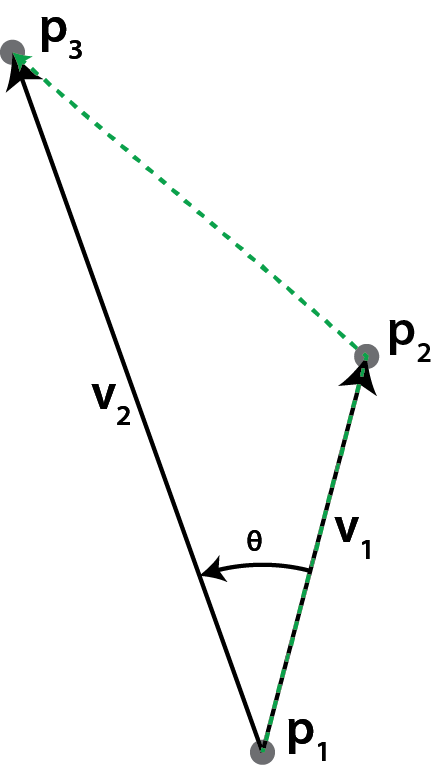
\includegraphics[width=0.9\textwidth]{./img/b_LeftTurn.png}
		\caption{left turn}
		\label{subfig:b:LeftTurn}
	\end{subfigure}
	\begin{subfigure}[b]{0.3\textwidth}
		\centering
		\includegraphics[width=0.9\textwidth]{./img/b_rightTurn}
		\caption{right turn}
		\label{subfig:b:RightTurn}
	\end{subfigure}	
	\begin{subfigure}[b]{0.3\textwidth}
		\centering
		\includegraphics[width=0.9\textwidth]{./img/b_noTurn}
		\caption{no turn}
		\label{subfig:b:NoTurn}
	\end{subfigure}		
	\caption{A path, the green dashed line, through the points $\vec{P_1}$, \vec{P_2} and \vec{P_3} making (\subref{subfig:b:LeftTurn}) a left, (\subref{subfig:b:RightTurn}) a right turn and (\subref{subfig:b:NoTurn}) no turn.}
	\label{fig:b:turns}
\end{figure}

\autoref{fig:b:turns} presents the three possible types of paths that form a straight line through the points $\vec{P_1}$, $\vec{P_2}$ and $\vec{P_3}$. Converting these three 2D points to three dimensional ones, by adding a $z$-coordinate that is zero, allows us to use the cross product to determine the angle $\theta$, using the definition of the cross product:

\begin{equation}\label{eq:b:crossProduct}
	\vec{v_1} \times \vec{v_2} = 
	\norm{\vec{v_1}} \cdot \norm{\vec{v_2}} \cdot \vec{n} \cdot \sin \theta.
\end{equation}
Where the $\vec{v_1} = \vec{P_2} - \vec{P_1}$, $\vec{v_2} = \vec{P_3} - \vec{P_1}$ and $\vec{n} = [0, 0, 1]$ represents the normal of the plane that contains the points. 

Since all values but the last of the vector \vec{n} are zero the result of \eqref{eq:b:crossProduct} will be of the form $[0, 0, q]$, where $q$ is influenced by $\sin \theta$. The norms of the vectors \v{1} and \v{2} are greater than or equal to zero by definition. And does not influence the value of $q$. From this we can conclude that the sign, or the lack thereof of $q$ is completely dependent upon $\sin \theta$. As we are only interested in the direction of the angle, not in its size we can use this to determine the type of path.\\

If the points are collinear the angle $\theta$ is $\pi$ and which results in $q = 0$. If $q$ is negative the path makes a left turn, if $q$ is positive the path makes a right turn.\\

Using Mathematica, see \autoref{lst:b:mat}, we get an expression for the value of $q$:
\begin{equation}\label{eq:b:q}
	q = -\p{1}_y \p{2}_x + \p{1}_x \p{2}_y + \p{1}_y \p{3}_x - \p{2}_y \p{3}_x - \p{1}_x \p{3}_y + \p{2}_x \p{3}_y,
\end{equation}
where $\p{1}_y$ represents the $y$-coordinate of the point \p{1}.

\begin{lstlisting}[float, language=Mathematica, label={lst:b:mat}, caption={Mathematica code used to compute the value of $q$.}]
p1 = {p1x, p1y, 0};
p2 = {p2x, p2y, 0};
p3 = {p3x, p3y, 0};

v1 = p2 - p1;
v2 = p3 - p2;

Cross[v1, v2]	
\end{lstlisting}

% To determine the type of turn, if any, a path makes we are interested in the sign of angle $\theta$, shown in \autoref{fig:b:turns}, for both a left turn (\protect\ref{subfig:b:LeftTurn}) and a right turn (\protect\ref{subfig:b:RightTurn}). Each point $\vec{P_r}$ represents the vector $[x_r, y_r]$, with $r \in \{1, 2, 3\}$. Representing each point $\vec{P_3}$ as a three-dimensional vector results in the vector $[x_r, y_r, 0]$. The vector $\vec{v_1}$ is defined as $\vec{P_2} - \vec{P_1}$ and $\vec{v_2} = \vec{P_3} - \vec{P_1}$.

% Now that we have these definitions we can use the equality in \eqref{eq:b:crossProduct} to determine the sign of $\theta$, which should tell us if the line through the points $\vec{P_1}$, $\vec{P_2}$, and $\vec{P_3}$ makes a left or a right turn, or no turn at all. 

% The vector $\vec{n}$ is the unit normal vector of the plane of the vectors $\vec{v_1}$ and $\vec{v_2}$, since all points lie in the $z$-plane $\vec{n} = [0, 0, 1]$. We use $\vec{q} = [a, b, c]$ to denote the result of the cross product of the vectors $\vec{v_1}$ and $\vec{v_2}$. Since the first two elements of the vector $\vec{n}$ are zero, $a$ and $b$ are also zero.

% The scalars $\norm{\vec{v_1}}$ and $\norm{\vec{v_2}}$ are by definition positive, as is the one provided by the normal vector. Thus only the factor $\sin \theta$ influences the sign of $c$.







\section{~}
\label{s:c}
%!TEX root = practicum3.tex
To find the intersected edges and compute the intersection points we have used the method \t{find_intersected_edges}, see \autoref{lst:c:find_intersected_edges}. This method calls the method \t{line_segments_intersect} (\autoref{lst:b:intersectLineSegments}) on the edge defined by the points \t{p0} and \t{p1} and the edges of the triangulation. If an intersection is found it adds the indices of the intersected edge in the global list \t{intersected_line_segments} and appends the intersection point to \t{intersection_points}. The intersected edges of the triangulation and the intersection points are presented in \autoref{tab:c:intersectedEdges}.

\lstinputlisting[float, firstline=180, lastline=199, label={lst:c:find_intersected_edges}, caption={The method \t{find_intersected_edges()}.}]{../assignment3C.py}

To visualize the results we have added the code in \autoref{lst:c:display_1}, the resulting visualization is shown in \autoref{fig:c:result}.

\lstinputlisting[float, firstline=115, lastline=129, label={lst:c:display_1}, caption={Part of the method \t{display()} that visualizes the intersected edges and the intersections.}]{../assignment3C.py}

\begin{figure}
	\centering
	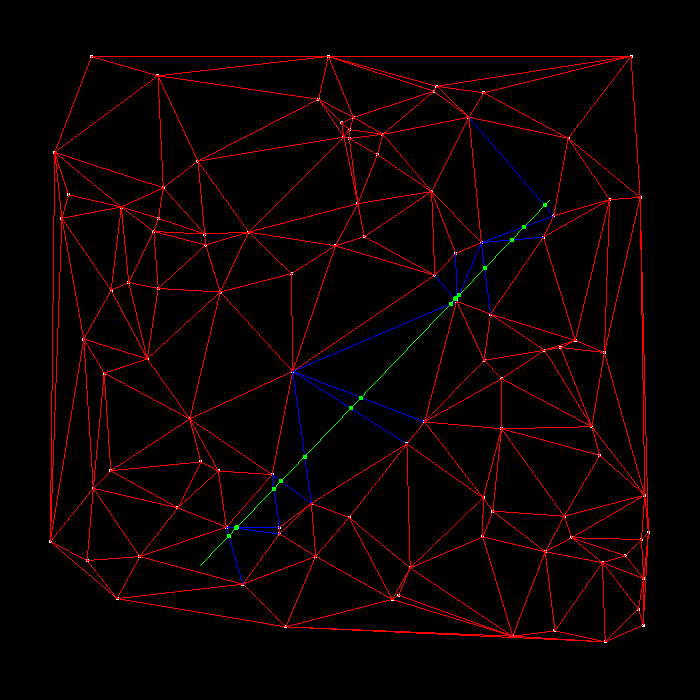
\includegraphics[width=0.5\textwidth]{./img/c_result}		
	\caption{The visualization of the intersection of the line segment $s$ with the edges of the triangulation $dt$. Each intersected edges is shown in blue, the green dots represent the intersections.}
	\label{fig:c:result}
\end{figure}


\begin{table}
	\centering
	\footnotesize{
		\begin{tabular}{ll|ll}
		edge & intersection & edge & intersection\\
		\hline
		(\num{226.33195013}, \num{527.007719279}) - (\num{242.796962849}, \num{584.179466813})	&	(\num{228.867696999}, \num{535.812636852})	&	 (\num{456.54758505}, \num{301.329564578}) - (\num{292.651351959}, \num{371.369188947})	&	(\num{450.717707067}, \num{303.820912038})	\\
		(\num{226.33195013}, \num{527.007719279}) - (\num{279.526723944}, \num{533.851551524})	&	(\num{236.087462036}, \num{528.262825414})	&	 (\num{434.746175446}, \num{275.228689898}) - (\num{456.54758505}, \num{301.329564578})	&	(\num{454.940291133}, \num{299.405295558})	\\ 
		(\num{226.33195013}, \num{527.007719279}) - (\num{279.230162351}, \num{527.629726937})	&	(\num{237.165877611}, \num{527.135110841})	&	 (\num{543.382588894}, \num{237.142130429}) - (\num{481.36728233}, \num{242.669629937})	&	(\num{511.78866886}, \num{239.958134849})	\\ 
		(\num{272.14012592}, \num{474.6185968}) - (\num{279.230162351}, \num{527.629726937})	&	(\num{274.010859273}, \num{488.60578716})	&	 (\num{481.36728233}, \num{242.669629937}) - (\num{490.590138248}, \num{314.176426186})	&	(\num{484.674568747}, \num{268.311736682})	\\ 
		(\num{272.14012592}, \num{474.6185968}) - (\num{311.312430627}, \num{503.369689707})	&	(\num{281.098731465}, \num{481.193897954})	&	 (\num{481.36728233}, \num{242.669629937}) - (\num{456.54758505}, \num{301.329564578})	&	(\num{459.283383215}, \num{294.863662123})	\\ 
		(\num{292.651351959}, \num{371.369188947}) - (\num{406.885957326}, \num{443.993258738})	&	(\num{350.781795159}, \num{408.325322776})	&	 (\num{455.757245676}, \num{253.484433518}) - (\num{456.54758505}, \num{301.329564578})	&	(\num{456.489045688}, \num{297.785740795})	\\ 
		(\num{292.651351959}, \num{371.369188947}) - (\num{311.312430627}, \num{503.369689707})	&	(\num{304.689843297}, \num{456.524335295})	&	 (\num{553.745608126}, \num{215.87226731}) - (\num{481.36728233}, \num{242.669629937})	&	(\num{524.448996513}, \num{226.719049361})	\\ 
		(\num{292.651351959}, \num{371.369188947}) - (\num{424.577450772}, \num{421.869738174})	&	(\num{361.075143445}, \num{397.561421426})	&	 (\num{468.981532514}, \num{117.202657047}) - (\num{553.745608126}, \num{215.87226731})	&	(\num{544.790307044}, \num{205.447850348})	\\	 	
		\end{tabular}
	}
	\caption{The edges that were intersected by the line segment between \t{p0} and \t{p1} and the point where the line segment intersected the edge. A point \vec{P} defined by its $x$ and $y$ coordinate is represented as $(x, y)$. A linesegment between the points \vec{P_1} and \vec{P_2} is represented as (\vec{P_1}, \vec{P_2}).}
	\label{tab:c:intersectedEdges}
\end{table}

~\\

\todo[inline]{Find and print the consecutive intersection points going from p0 to p1 without using the actual coordinates of the intersection points.}




\end{document}